\documentclass[11pt]{article}
\usepackage{amssymb}
\usepackage{amsmath}
\usepackage{mathrsfs}
\usepackage{graphicx}
\usepackage{float}
\usepackage{hyperref}
\usepackage{breakurl}
\graphicspath{ {./images/} }

\begin{document}
	\pagenumbering{gobble}
	\title{Embedded System 1 Project \\
		\large UART exploration, frame decoding \\and Hamming code error correction}
	
	\author{Alberto Tiraboschi \\ Email: \href{mailto:alberto1.tiraboschi@mail.polimi.it}{alberto1.tiraboschi@mail.polimi.it} \and Alessandro Andrea Vogrig \\ Email: \href{mailto:alessandroandrea.vogrig@mail.polimi.it}{alessandroandrea.vogrig@mail.polimi.it}}
	\date{}
	\maketitle
	\thispagestyle{empty}
	\clearpage
	\tableofcontents
	\thispagestyle{empty}
	\cleardoublepage	
	\pagenumbering{arabic}% Arabic page numbers (and reset to 1)

	\section{Introduction}
	During the development of softwares for simulated hardware on Vivado, it sometimes happens that the module UART is chosen to carry out communications to other devices rather than to the user. If we consider an hardware simulated by software on Vivado, no practical system to decode inbound (RX) or outbound (TX) UART signals is observed. To simplify the data transmission debug on UART, we have decided to develop a module which is able to run the decodification process of the RX and TX signals; in this way human interaction is possible. To increase the reliability level of the long-distance transmission, we have also developed a module which can evaluate 4+1 bit more than the simple parity bit; as a consequence, in addition to the error detection, we can also carry out the error correction on errors on a single or two bits and signal an error over errors with more bit. The UART\_0 module is transparent with respect to the final users of the transmission, so that it can be used without necessarily acting on the software side for correct data transmission. \\
	Even if only tested on Cortex M3 and AXI UART Lite, the module developed by us should not theoretically have compatibility problems with other implementations, as it is independent of the ARM architecture used.
	
	\section{System analysis}
	\subsection{UART Lite}
	To better understand what led us to make certain design choices, an overview of the operation of UART serial communication on devices based on ARM Cortex M3, AXI Interconnect and AXI UART Lite is given.
	\begin{figure}[H]
			\begin{center}
		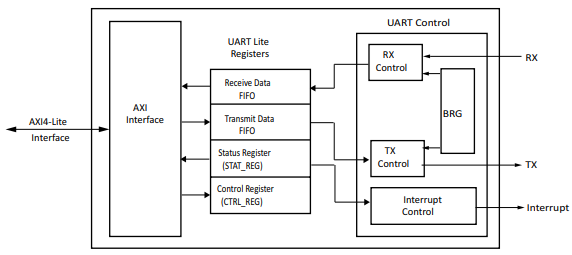
\includegraphics[scale=0.80]{AXI_UART_Module}	
		\caption{AXI UART Lite module block diagram}
	\end{center}
\end{figure}
	As Figure 1 shows, the module consists of 4 channels, 2  of which are used for communication with the processor (labeled "AXI4-Lite Interface" and "Interrupt") and the remaining 2 for communication from and to the outside (RX and TX). In the implementation of the device taken as an example, the RX and TX signals are not directly exposed to the outside of the device, but are sent to the DAP-Link module with the function of debugger and programmer that takes care of retransmitting them externally. The usefulness of this module is limited to us in a simulated environment such as the one considered. Therefore, its function was not investigated. \\
	The module can be divided into three main sub-blocks:
	\begin{itemize}
	\item AXI Interface: implements the slave mode functions of the AXI4 Lite protocol to allow communication to and from the processor of data and settings.
	\item UART control: takes care of generating and decoding the UART signals on the TX and RX lines, respectively. The BRG (baud rate generator) block is responsible for generating the necessary clock to maintain the set transmission speed (baud rate). The interrupt generator (interrupt control) generates two different kinds of interrupt signals (rising edge) on the same line for the processor: in the case of new data available in the reception queue (Receive data FIFO), they are particularly useful, if you want to avoid polling the CPU and to probe the presence of any new data received from the outside (through the RX line) and if the transmission queue (Transmit data FIFO) is not full, to invite the CPU to send new data to be transmitted.
	\item UART Lite registers: are the registers useful for the functioning of the module.
	\end{itemize}
	Access to the registers is direct and defined by memory offset with respect to the module base address.
	The available registers are:
	\begin{itemize}
	\item RX FIFO: 16-level queue containing received data. This is a read only register, any write requests are ignored;
	\item TX FIFO: 16-level queue containing the data to be sent through the UART module. The register is write only. If an attempt is made to write while the register is full, an error flag is set into the status register;
	\item Control register (CTRL\_REG): it is a write only register through which you can enable or disable the interrupt output of the module and empty the RX FIFO and TX FIFO registers through reset commands;
	\item Status register: (STAT\_REG): it is a read only register that contains the status of the FIFO registers and flags any errors. In particular, there is a bit to identify an error in the parity bit in received packets, a bit to identify malformed frames, a bit to report received and discarded data due to the full reception queue and 4 bits to report the status of the reception and transmission queues.
	\end{itemize}
	In the AXI\_Uart\_Lite module, the transmission speed, size and characteristics of the frame are established with a special tool to customize the IP when the module is generated. Therefore, they cannot be modified through software at the time of execution. For this reason, our implementation choice has focused on an 8-bit packet without parity bit and a transmission speed of 115200 baud/s. It remains possible to modify and adapt our solution for other frame rates and formats with minimal changes.
	\subsection{System overview}
	With the  help of the block diagram of the ARM M3 core implementation, we illustrate how the processor can manage UART communications.\\
	\begin{figure}[H]
	\centering
	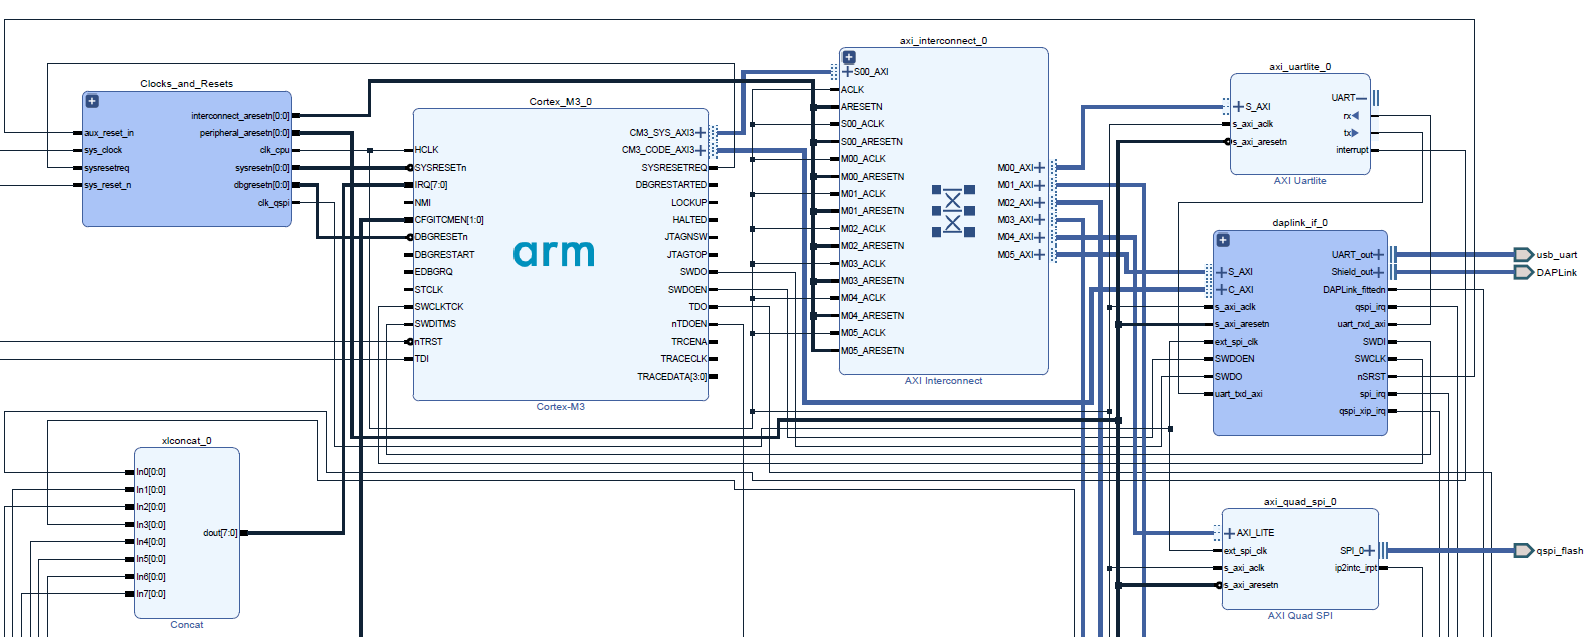
\includegraphics[height=0.55\textwidth, angle=90]{M3_block}
	\caption{overview of AXI UART module implementation}
	\end{figure} 
	
	There are mainly two ways in which the processor can read and send data to the UART module: by polling or by exploiting interrupts.\\
	If the processor wants to transmit a byte on the UART TX port, it must send a write request to the TX FIFO register address, passing through AXI Interconnect. However, this procedure can only take place provided that the transmission queue is empty. The processor must first make sure of this by checking the status register of the AXI UART Lite module. In polling mode, this check is performed at regular intervals, by sending requests to read the STAT\_REG register and by checking that the queue full flag is not set. On the other hand, if you choose to exploit the interrupts, the UART module would signal an interrupt, raising the appropriate line; at this point, the processor can check the status register of the module to verify the buffer condition  and, subsequently, send the data to be written, avoiding numerous empty queries of the status register. \\
	The data reception process is similar to the transmission one: once a packet has arrived on the UART RX line and after any checks on the parity bit, the received byte is inserted in the RX FIFO reception queue and the appropriate bit indicating valid data received in the status register is brought to 1. Thereafter, you can proceed in two ways: by polling or by exploiting interrupts.
	In the first case, the processor will have to periodically check the status register in order to detect the presence of new bytes in the reception queue which it will have to read with a further request. In the latter case, the processor will check only when an interrupt is triggered. \\
	It is important to notice that, even by exploiting interrupts, the processor should always check the status register;   whether it is generated by the transmission process or by the receiving one, the interrupt is unique, so  it is not possible to distinguish them beforehand.
	\section{Alternative analysis}
	Given our premises, possible alternatives to the one actually implemented are illustrated below. \\
	The primary purpose of this solution is to provide an easy way for the person to decode what is sent and received in a UART communication.
	This operation should ideally be performed without significantly modifying the existing hardware implementation; this leads to the elimination of any solution that directly modifies the AXI\_UART\_Lite module. The intention, in fact, is to provide a decoding tool for an existing hardware implementation, so that even the software compiled for it does not have to undergo any changes.
	Such a decoding operation can be performed by a module connected mainly by three different points: it is possible to connect to the AXI bus between the processor and AXI Interconnect, to the bus between AXI inteconnect and the AXI UART Lite module or to the RX and TX lines.
	It should be noted, however, that using the bus between the processor and AXI Interconnect as a data source for the module would inevitably lead to the latter adding complexity due to the need to filter all requests not intended for the UART module. Furthermore, if not carefully designed, the module could cause a bus overload due to the added parasitic capacities, undermining the correct functioning of the entire system.
	Another possibility is to connect the decoding module between AXI Interconnect and the AXI UART Lite module. This option is also suboptimal: it partially solves the problem of request filtering, but does not eliminate the risk of overloading the line. Furthermore, an AXI-based approach would make it very difficult to realize the secondary purpose of this project: a transparent correction of single-bit errors in the packet using Hamming encoding.\\
	The creation of an external module, which uses only the TX and RX lines, brings numerous advantages over the previous solutions: it is not necessary to perform any filtering of the data read, since they are exactly the packets to be decoded; UART lines are more tolerant of parasitic capacitance than the AXI bus, and, in the case of a physical implementation, it would be easy to add buffers to compensate for these additional loads. The realization of a module totally independent from the already present system allows to leave the RX and TX signals unchanged, which can be used for other purposes. Furthermore, being an external and independent module, portability to other devices is considerably simplified, requiring only the two RX and TX signals present in each UART communication.		
	An example usage scenario is graphically summarized below:\\
	\begin{figure}[H]
	\begin{center}
		
\includegraphics[scale=0.35]{diagram 1}	
		\caption{schematic implementation of the modules}	
	\end{center}
	\end{figure}
	On the right and left there are two microcontrollers (MC1, MC2), in the middle a simplified representation of the developed UART\_0 modules. The transmission starts from MC1, which reaches the immediately connected module. The communication between this and the UART\_0 module at the other end of the communication takes place by adding parity bits according to the Hamming scheme. The target module will receive the packet, correct (where possible) the packet, or alternatively report a packet problem externally, causing an interrupt in the MC2 microcontroller. By configuring a precedence on the interrupt order, the signal will be intercepted before the packet is received, allowing the receiver to signal in good time the re-sending of the wrong packet to the sender MC1.
	
	\section{Description of the designed module}
	\begin{figure}[H]
	\begin{center}
		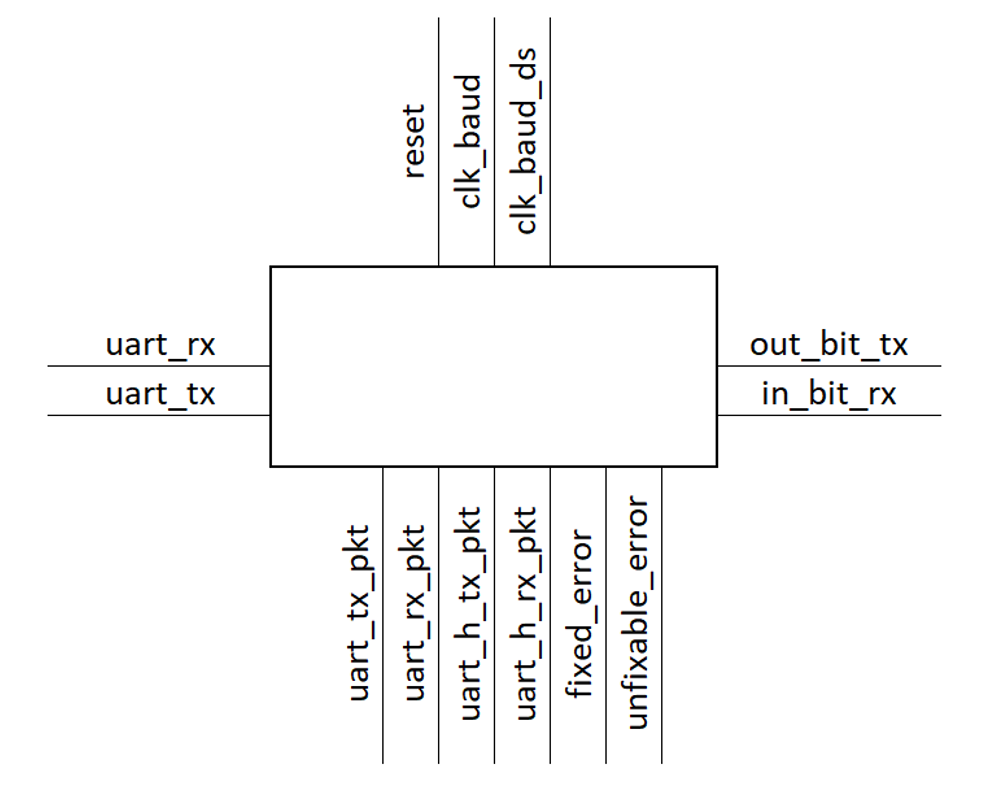
\includegraphics[scale=0.5]{module schem}
		\caption{designed module}	
	\end{center}
	\end{figure}
	The main lines are:
	\begin{itemize}
		\item uart\_tx and uart\_rx: connections to UART module;
		\item out\_bit\_tx and in\_bit\_rx: connections between two UART\_0 modules carrying a UART packet with Hamming code;
		\item fixed\_error and unfixable\_error: used to signal to the microcontoller a fixed or unfixable error.
	\end{itemize}
	The module is activated in one of the following cases:
	\begin{itemize}
	\item There are bits in on uart\_rx at clk\_baud speed;
	\item There are bits coming into in\_bit\_rx at clk\_baud\_ds speed.
	\end{itemize}
	In the first case, the packet (8 fixed bits for simplicity, but extendable to a certain parameter), recognized by the initial bit at zero, is inserted into a new packet, which contains the bits according to the Hamming scheme, shown here below (with a final parity bit on all bits (including Hamming parity bits)):
	\begin{figure}[H]
	\begin{center}
		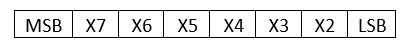
\includegraphics{p1}		
	\end{center}
	\end{figure}
	\begin{figure}[H]
	\begin{center}
		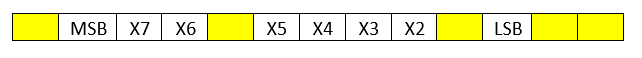
\includegraphics{p2}		
	\end{center}
	\end{figure}
	This packet is reported on the uart\_h\_tx\_pkt bus, while the original is reported on the uart\_rx\_pkt bus.
	In the second case, the packet (reported on the uart\_h\_rx\_pkt bus), already in the form with Hamming, is first decoded, then corrected (where possible) and finally the result is reported on uart\_tx\_pkt. By calling P, the XOR of all the bits of the received packet (13) and C, the count given by the positions of the Hamming bits that do not match, the following table can be used for the error checking procedure:
	\begin{center}
		\begin{tabular} {|c|c|c|}
		\hline
		C & P & Outcome\\
		\hline
		\hline
		= 0 & 0 & No errors\\
		= 0 & 1 & Error on the bit 13. Can be fixed.\\
		$>$ 0	& 1	& Single bit error. Can be fixed\\
		$>$ 0 & 0 & Double error. Cannot be fixed.\\
		\hline
		\end{tabular}
	\end{center}
	As it can be seen from the last two columns of the table, it is necessary to add the final parity bit in order to understand whether it is possible to correct the error.
	Depending on the type of error, a signal is sent outside to notify the user and/or connected devices of the outcome of the procedure.
	The packet is finally transmitted on uart\_tx and returns to the sender with the same baud\_rate with which it sends messages. The modules in between to avoid the formation of queues work at double baud\_rate.
	\begin{figure}[H]
				\begin{center}
		
		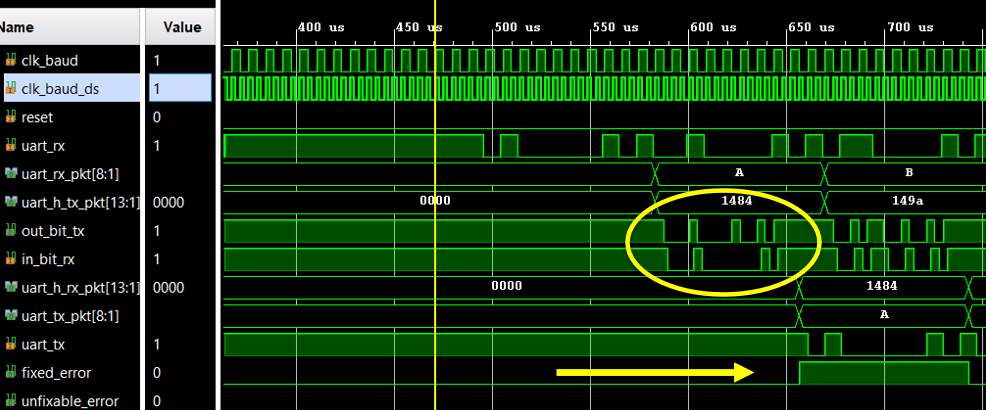
\includegraphics[scale=0.65]{1 error}	
				\caption{fixable error detection and correction}
			\end{center}
	\end{figure}
	\begin{figure}[H]
		\begin{center}
		
		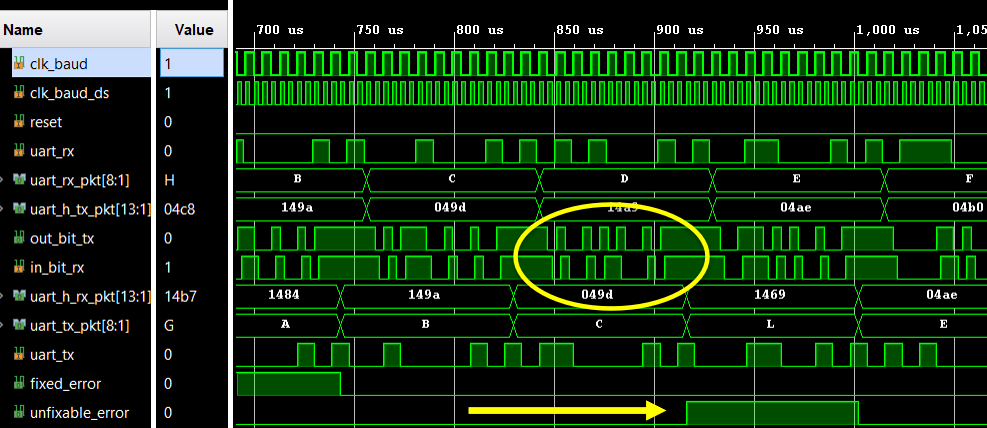
\includegraphics[scale=0.65]{2 errors}	
				\caption{unfixable error detection signaling}	
			\end{center}
	\end{figure}
	\clearpage
	\section{Bibliography}
	\begin{itemize}
		\item
		\url{https://www.xilinx.com/support/documentation/ip_documentation/axi\_uartlite/v2_0/pg142-axi-uartlite.pdf}
		\item \url{https://www.xilinx.com/support/documentation/ip_documentation/axi_ref_guide/latest/ug761_axi_reference_guide.pdf}
		\item \url{https://en.wikipedia.org/wiki/Hamming_code}
		\item \url{https://www.youtube.com/channel/UCIrNyLpdgJRkBLOf-V7L93g}
		\item \url{https://developer.arm.com/ip-products/designstart/fpga}
	\end{itemize}

\end{document}